\section{Introduction}
Nowadays when surfing the web CAPTCHA tests are everywhere, to the point we are used to get asked to prove our humanity and something is off when it does not happen.
Furthermore, technology moves forwards and tests are becoming increasignly harder, while it may be a nuisance for the abled it can often be a barrier for people with disabilities.
It is a priority to develop reliable CAPTCHA tests designed to be accessible to everyone.

The word CAPTCHA stands for \emph{Completely Automated Public Turing test to tell Computers and Humans Apart}.
In the year 2000 during a speaking at Carnegie Mellow University held by YAHOO!, at the time one of the world's biggest companies, they listed the ten most relevant problems they did not know hot to solve; among these issues stood out that spammers would write programs to automatically generate mails, and use them for malicious purposes~\cite{vox2021captcha,theverge2019captcha}.
The world needed a test to distinguish humans from computers such that any human, regardless of age, gender, education or language could pass it.
To make things even more difficult, the CAPTCHA test is born from a paradoxical idea: any computer should be able to grade it but should not be able to pass it, like if a teacher could grade students' exams without knowing the subject.

\paragraph{CAPTCHA}
The idea exposed in \cite{vonahn2003captcha} is based on the fact that humans are extremely good at pattern and optical character recognition i.e., reading, and we
generally learn to do it since we are kids and can do it under many circumstances like bad lighting and other.
A text is took and warped, stretched or generally modified in some way such tha computer vision techniques at the time could not read it, yet the computer with the gold truth just has to match it with the user's input.
Once released CAPTCHA has been used to authenticate access to YAHOO! mail services.

\paragraph{reCaptcha}
All the character input by humans into CAPTCHA gave new data that made computers smarter.
The new versione, reCAPTCHA~\cite{ahn2008recaptcha}, uses two words: one generated so the compute knows the answer and the other pulled from a book or originally a \emph{The New York Times}' old article, both of which are distorted.
When a human gets the first word right the system guesses the second one is probably right and distributes it across different users, if there is consensus then it is approved.
So many tests were done that something along one year of NY Times articles was digitalized every 4 days, this led Google to acquire reCAPTCHA in 2009 and exploit it to digitalize texts in its archive.
When you do that enought times you get a big enough dataset of distorted characters that computers can effectively learn how to read them, in a way CAPTCHA taught machines how to read highly warped texts, in a 2014 machine learning study Google stated how humans have a 33\% accuracy on recognizing CAPTCHA's warped characters while a trained machine has 99.8\%~\cite{google2014recaptcha}.

\paragraph{reCAPTCHAv2}
Given the huge potential reCAPTCHA showed to have, Google exploited it to have human users classify images and build up a data, that were later used to improve Google Maps~\cite{vox2021captcha}.
Again, computers eventually became good enough on images that reCAPTCHAv2 is not enough anymore.

\paragraph{NoCAPTCHA reCAPTCHAv3}
Computers changed and tests have to change as well, NoCAPTCHA reCAPTCHAv3~\cite{google2014nocaptcha} are behavioral-based: a background test is always running and if it detects some bot-like behavior e.g., clicking around or writing large chunks of text in a very short time, it makes you take a standard test.
Alternatively, instead of a test it aks for authentication, based on the idea that is possible to tell you are not a robot given that is possible to tell who you are.

\begin{figure}[h!t]
    \centering
    \begin{subfigure}{0.49\textwidth}
        \centering
        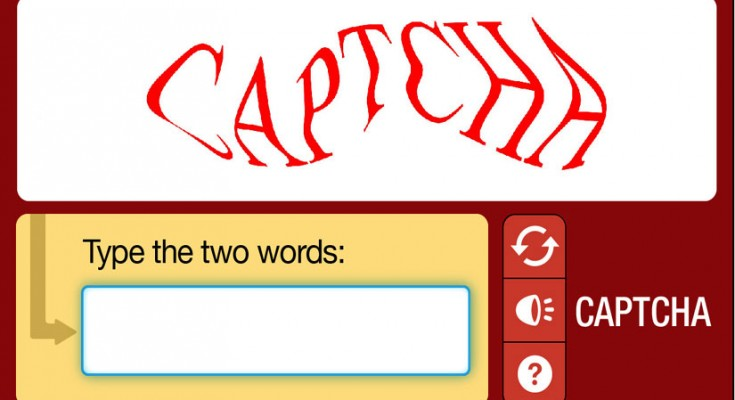
\includegraphics[scale=0.2]{assets/images/captcha.jpg}
        \caption{CAPTCHA.}
        \label{fig:captcha:catpcha}
    \end{subfigure}
    \begin{subfigure}{0.49\textwidth}
        \centering
        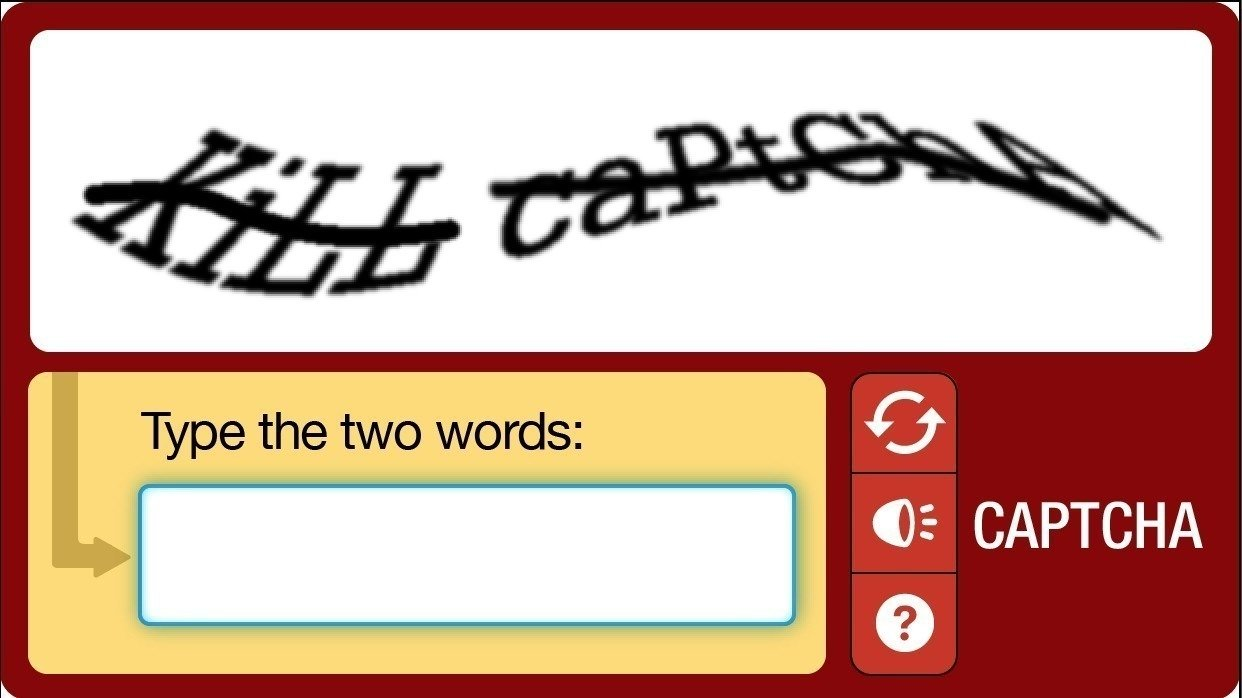
\includegraphics[scale=0.23]{assets/images/recaptcha.jpg}
        \caption{ReCAPTCHA.}
        \label{fig:captcha:recatpcha}
    \end{subfigure}
    \begin{subfigure}{0.49\textwidth}
        \centering
        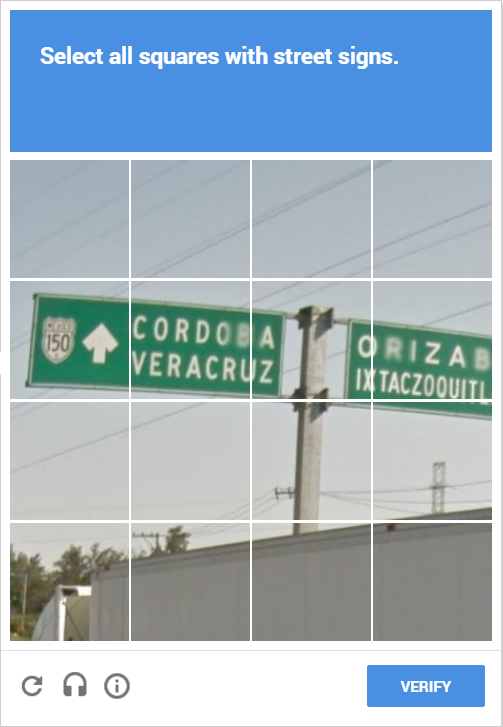
\includegraphics[scale=0.25]{assets/images/recaptchav2.png}
        \caption{ReCAPTCHAv2.}
        \label{fig:captcha:recatpchav2}
    \end{subfigure}
    \begin{subfigure}{0.49\textwidth}
        \centering
        
\includegraphics[scale=0.25]{assets/images/nocaptcha.jpg}
        \caption{NoCAPTCHA.}
        \label{fig:captcha:nocatpcha}
    \end{subfigure}
    \caption{Visualizationof the different CAPTCHA tests presented in this historical review.}
    \label{fig:captcha}
\end{figure}

The CAPTCHA problem is far from solved and, realistically, at some point the current CAPTCHA test will be obsolete.
A problem present in all the test instances we saw is accessibility e.g., no deafblind person could pass one of them.
Speaking from personal experience, while surfing the web I noticed that there are very few options for disabled people: once I found the possibility to select an audio test but still the default selection was a classical visual CAPTCHA.